\documentclass[11pt]{beamer}
\mode<presentation>
\let\Tiny=\tiny
\usetheme{CambridgeUS}
\usefonttheme{professionalfonts}
\usepackage[brazil]{babel}
\usepackage[utf8]{inputenc}
\usepackage{amsfonts}
\usepackage{amssymb}
\usepackage{amsmath}
\newtheorem{mydef}{Definição}
\newtheorem{myexample}{Exemplo}

\title{Prototipação}
\author{}
\date{}

\begin{document}

    \begin{frame}[plain]
        \titlepage
    \end{frame}

    \section{Introdução}

    \begin{frame}{Prototipação}
      \begin{itemize}
        \item Produtos inovadores são trazem consigo um grande risco, pois estão em fronteiras pouco exploradas.
        \item Surge a necessidade de provar que a ideia por trás desses produtos realmente funciona.
      \end{itemize}
    \end{frame}

    \begin{frame}{Prototipação}
      \begin{itemize}
        \item O uso da técnica de prototipação permite que as empresas testem rapidamente suas ideias.
        \item Uma ideia testada trás mais segurança para investidores e até mesmo para os funcionários da empresas.
        \item Do parte dos funcionários, se o protótipo garante o produto, isto pode ser um indicativo de estabilidade (por algum tempo) para os envolvidos na construção do produto. 
      \end{itemize}
    \end{frame}

    \begin{frame}{Prototipação}
      \begin{itemize}
        \item Os protótipos podem ser classificados em 2 ou mais tipos (a depender do autor).
        \item Os mais comuns são os \textbf{descartáveis} e os \textbf{evolucionários}.
      \end{itemize}
    \end{frame}

    \begin{frame}{Prototipação}
      \begin{itemize}
        \item Os protótipos descartáveis são utilizados para testar ideias dentro do processo.
        \item Usos comuns dos protótipos descartáveis envolvem a criação de \textit{interfaces} e o teste de eficiência de algoritmos em determinadas situações.
        \item Como o nome já diz, estes protótipos são descartados assim que terminam os testes.  
      \end{itemize}
    \end{frame}

    \begin{frame}{Prototipação}
      \begin{itemize}
        \item Os protótipos evolucionários são utilizados mais largamente nas áreas de pesquisa e desenvolvimento.
        \item Na indústria automobilista e aeroespacial é comum a criação de protótipos de novos carros ou aeronaves para testar elementos como segurança, eficiência energética, etc.
        \item Para o desenvolvimento de \textit{software}, o uso de protótipos evolucionários é utilizado para apresentação a investidores ou com intuito científico.
        \item Diferentemente dos protótipos descartáveis, os protótipos evolucionários são mais robustos e bastante mais caros.
        \item Eles são construídos por etapas, agregando a cada iteração mais elementos.
      \end{itemize}
    \end{frame}

    \section{Prototipação no \textit{design} de \textit{interface}}

    \begin{frame}{Prototipação}
      \begin{itemize}
        \item Dificilmente o desenho ideal será atingido em um primeiro momento.
        \item O projeto de \textit{interface} tende a mudar diversas vezes até que se atinja o resultado ideal.
        \item A interação com seres humanos não é algo tão preditível.
        \item O uso de protótipos descartáveis hoje é comum na indústria de desenvolvimento de \textit{software}.
      \end{itemize}
    \end{frame}

    \begin{frame}{Prototipação}
      \begin{itemize}
          \item A prototipação pode ser incluída em diversas fases do ciclo de desenvolvimento, especialmente nas fases iniciais, quando há maior incerteza.
          \item Para cada \textit{user story} a ser implementada, deve-se especificar melhor seu fluxo de execução.
      \end{itemize}
    \end{frame}

    \begin{frame}{Prototipação}
      \begin{itemize}
          \item O fluxo de execução pode ser estabelecido por diferentes ferramentas.
          \item Algumas destas são: o \textbf{diagrama de atividades}, a \textbf{análise de tarefas} e os \textbf{storyboards}.
          \item Os dois primeiros são os mais próximos dos desenvolvedores de \textit{software}, enquanto o último é mais utilizado por artistas visuais.
      \end{itemize}
    \end{frame}

    \subsection{Análise de tarefas}

    \begin{frame}{Análise de tarefas}
      \begin{itemize}
          \item A análise de tarefas é uma "prática abrangente de aprender como os usuários trabalham ... para alcançar seus objetivos" (Rosala, 2020, trad. nossa)
          \item Tarefa é uma ação observável que possui um início e um fim definidos.
      \end{itemize}
    \end{frame}

    \begin{frame}{Análise de tarefas}
      \begin{itemize}
          \item Não se deve confundir uma tarefa com o objetivo.
          \item Se o objetivo é cadastrar-se em um \textit{site}, preencher o formulário de cadastro é uma atividade para atingir esse objetivo e não um objetivo em si.
      \end{itemize}
    \end{frame}

    \begin{frame}{Análise de tarefas}
      Tenha-se a \textit{user story}:
      
      "Eu, enquanto professor, desejo publicar aulas adaptadas para que os alunos surdos e não-surdos possam rever o conteúdo."

      A \textit{user story} em si é um objetivo.
    \end{frame}

    \begin{frame}{Análise de tarefas}
      \begin{itemize}
        \item Apenas a \textit{user story} não diz como este objetivo será realizado.
        \item É necessário decompô-la em tarefas intermediárias a serem realizadas.
      \end{itemize}
    \end{frame}

    \begin{frame}{Análise de tarefas}
      Para a \textit{user story} apresentada, é um exemplo de análise de tarefas:
      \begin{enumerate}
        \item Autenticar-se na plataforma.
        \item Ir à página de adicionar aula.
        \item Preencher o formulário com título da aula, disciplina, comentário.
        \item Subir vídeo da aula e material de apoio.
        \item Pressionar botão confirmar.
      \end{enumerate}
    \end{frame}

    \begin{frame}{Análise de tarefas}
      A partir das tarefas levantadas é possível já ter noção de alguns elementos de \textit{interface} que estarão presentes:
      \begin{itemize}
        \item botão para ir à página de adicionar aula (possivelmente estará presente em um \textit{menu});
        \item uma página específica para adicionar aula;
        \item um formulário com os campos título da aula, disciplina e uma caixa de texto de comentário;
        \item campos para subir vídeo da aula e material de apoio;
        \item botão para confirmação de publicação da aula. 
      \end{itemize}
    \end{frame}

    \subsection{Protótipos em papel}

    \begin{frame}
      \frametitle{Protótipos em papel}
      \begin{itemize}
        \item Os protótipos descartáveis mais simples são os protótipos em papel.
        \item Os protótipos em papel simulam não apenas o fluxo, mas definem elementos de \textit{interface}.
      \end{itemize}

      \begin{figure}[ht]
        \centering
        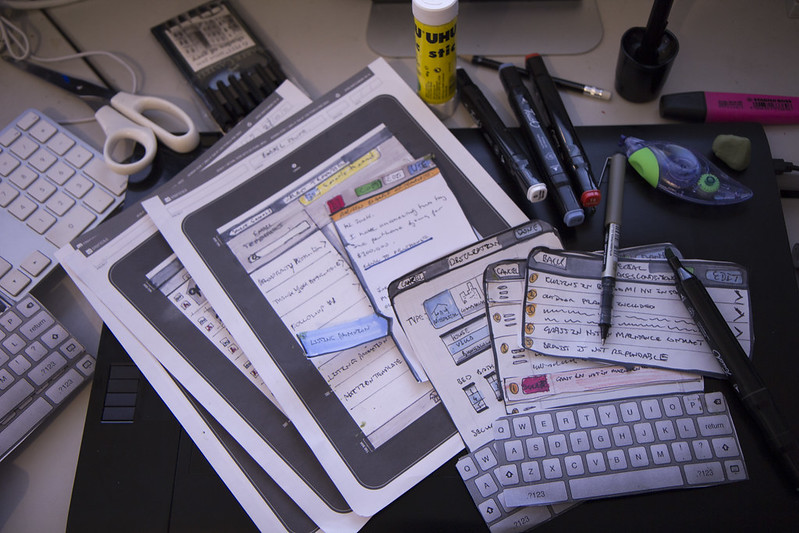
\includegraphics[height=5cm, width=8cm]{figures/paper_prototype.jpg}
        \footnote{Fonte: Flickr/CannedTuna. Licença: CC BY-NC-ND 2.0}
      \end{figure}
    \end{frame}

    \subsection{Protótipos digitais}

    \begin{frame}
      \frametitle{Protótipos digitais}
      \begin{itemize}
        \item Outro tipo de protótipo descartável são os protótipos digitais.
        \item Este tipo de protótipo são mais caros e exigem mais tempo para sua criação em relação aos protótipos em papel.
        \item Os protótipos digitais são protótipos que podem ser feitos utilizando ferramentas gráficas como Photoshop, Gimp, Sketchup ou Figma.
        \item Seu objetivo é permitir que os envolvidos comecem a visualizar a disposição dos elementos de \textit{interface} na tela.
      \end{itemize}
    \end{frame}

    \begin{frame}
      \frametitle{Protótipos digitais}
      É possível observar um exemplo de protótipo digital para um sistema de transporte em:

      https://1qcbl7.axshare.com/\#p=home\_screen
    \end{frame}

    \begin{frame}{Referências}
      \begin{itemize}
        \item Dix, Alan \textit{et al.}. Human-Computer Interaction. 3ed. Pearson Education. 2004.
        \item Rosala, Maria. Task Analysis: Support Users in Achieving Their Goals. 2020. https://www.nngroup.com/articles/task-analysis/
      \end{itemize}
    \end{frame}

\end{document}